% Chapter Template

\chapter{Monitoring Tool - Architecture} % Main chapter title

\label{Chapter3} % Change X to a consecutive number; for referencing this chapter elsewhere, use \ref{ChapterX}

\lhead{Chapter 3. \emph{Monitoring Tool - Part 1}}
\section{Requirements}
The first step of conception was to define the main goals of the system. This means enumerate all the features the people that will use it in the future really want and need. To structure our reflection, we used a pseudo version of the \emph{Goal Model} taught by Professor van Lamsweerde \cite{van2009requirements}. We tried to stay as close as possible to the original syntax but we may have taken some freedom to keep things simple.

\subsection{System Goals}
The main goal, as suggested by the title of the thesis, is to monitor and analyze a large WiFi network. We want to be able to know what happens currently on the network and understands the data generated by the all the network components. To achieve that we need to understand what the controller says in its log files and what are the data available in its \emph{Management Information Base}. 

Monitoring is also an active task. We shall need to analyze the quality of service experienced by a user when he uses the WiFi network on the UCL's campus. Besides the gathering part, we also have to analyze those results and moreover, we have to be able to detect issues as soon as possible.

\begin{figure}[H]
\centering
	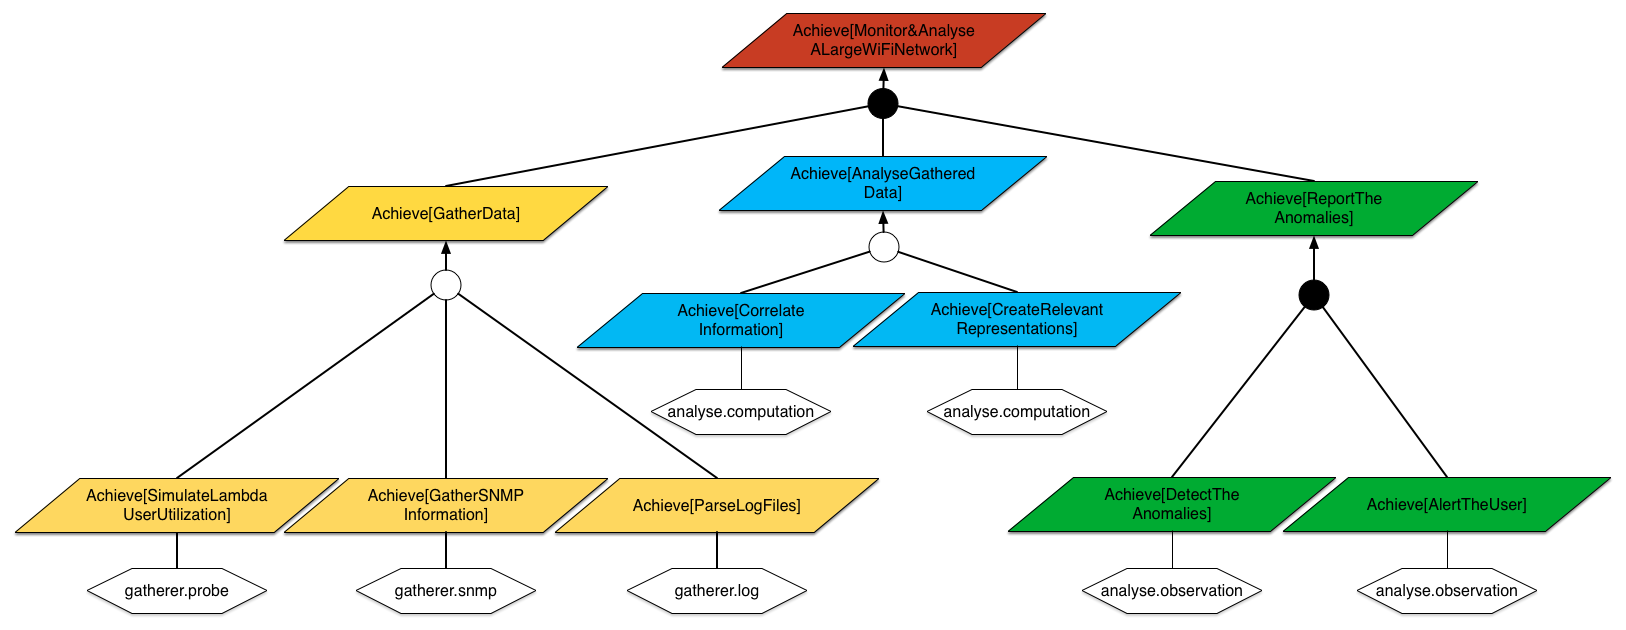
\includegraphics[width=1.1\linewidth]{Pictures/chapter3/goals2.png}
	\caption{Pseudo Goal Model}
\end{figure}

All these requirements come from the meetings we had with the SGSI during the implementation of this monitoring tool. We discussed about what sources of data we could use for this monitoring system and what are the information we could deduct from these data and from the analysis the tool can perform on them. It is quite important to determine what we are the goals and how we will achieve them. This rather simple model allows us to focus on one task at a time without loosing the final purpose of this project.

\subsection{Goals Definition}
\begin{description}
  \item[Name] Monitor\&AnalyseALargeWifiNetwork
  \item[Description] The root goal of our system is to allow the administrators to understand what is currently happening on the WiFi network.
\end{description}

\begin{description}
  \item[Name] GatherData
  \item[Description] To provide an efficient monitoring we have to gather and centralize all the available information. 
\end{description}

\begin{description}
  \item[Name] SimulateLambdaUserUtilization
  \item[Description] We need to evaluate how the users are experiencing the utilization of the network.
\end{description}

\begin{description}
  \item[Name] GatherSNMPInformation
  \item[Description] We have to record the states of the Controller and the access points through time using the \texttt{SNMP} protocol.
\end{description}

\begin{description}
  \item[Name] ParseLogFiles
  \item[Description] We have to be able to understand the information generated by the Controller, \texttt{RADIUS} and \texttt{DHCP} servers.
\end{description}

\begin{description}
  \item[Name] AnalyseGatheredData
  \item[Description] Once data are available, we need to analyze them and make comparison between them.
\end{description}

\begin{description}
  \item[Name] CorrelateInformation
  \item[Description] We want to put related data together in order to generate new information.
\end{description}

\begin{description}
  \item[Name] CreateRelevantRepresentations
  \item[Description] Our results have to be understood by the users through relevant and dynamic graphical representations.
\end{description}

\begin{description}
  \item[Name] ReportTheAnomalies
  \item[Description] More than analyzing data, the system has to be able to alert the administrators of anomalies.
\end{description}

\begin{description}
  \item[Name] DetectTheAnomalies
  \item[Description] Anomalies have to be defined precisely and the system has to use those rules to record deviant network behaviors.
\end{description}

\begin{description}
  \item[Name] AlertTheUser
  \item[Description] The system communicate and displays the anomalies to the users.
\end{description}


\section{Architecture}
In our architecture system, we have two very distinct entities. The first entity, called the \textit{Gatherer}, is the one responsible for gathering information. This component handles the responsibility to keep the operational database up to date and in a consistent state. The other side of the application, the \textit{Analyzer}, is managing the analysis process made with all the information we have gathered. Upon these two processes, we'll add an alert system that produces warnings when an anomalies is spotted. These three parts have to be as independent as possible but also have to be able to communicate between them efficiently. We have designed them by keeping two rules in mind: modularity and simplicity.

\subsection{Gatherer}
This part of the application is constituted of several modules that allow it to communicate with the various sources of information. Each module is responsible of a particular kind of information and each of them have to transform that piece of information in a coherent entry in the database. As the information come from heterogeneous origins, each information have to be understood and transformed into an entity that can be related to others. Without such transformation, the possible analysis would be really limited and not really interesting. We focus here on the \texttt{Achieve[GatherData]} goal and its refinement.

\subsubsection{Logs}
The first kind of information we analyzed was the log files. For each component of the infrastructure there is a different type of log. As a reminder, these are the three main components:
\begin{itemize}
\item RADIUS
\item DHCP
\item WiSM (Controller)
\end{itemize}
These elements generate several logs each seconds and the main difficulty is to make a first sorting process among all those data. A part of them is just informational and does not bring any useful information about the state of the network. Such messages will never be used during the analysis and then they do not need to be stored in the database. Another part of the logs are just repetition of others. In fact, as each element produces its logs independently, some logs can overlap and represent the same information. Redundant information are useless and the same information does not need to be stored twice in the database. This might seem to be an negligible issue but in consideration of the quantity of information proceeded by the application, an overloading of the database can cause severe performance issues during the analysis phase. For example, we can see that each time we have two logs \texttt{\%APF-6-RADIUS\_OVERRIDE\_DISABLED}, a third \texttt{\%LOG-6-Q\_IND} appears. That's typically the kind of sorting process we perform during the parsing.\\

\begin{lstlisting}[frame=single,breaklines=true,caption={Example of useless WiSM logs}]
2013-10-21T17:26:00.957695+02:00 192.168.251.178 WiSMPythagore-B: *Dot1x_NW_MsgTask_0: Oct 21 17:26:00.915: %APF-6-RADIUS_OVERRIDE_DISABLED: apf_ms_radius_override.c:204 Radius overrides disabled, ignoring source 2 
2013-10-21T17:26:00.958457+02:00 192.168.251.178 WiSMPythagore-B: *Dot1x_NW_MsgTask_0: Oct 21 17:26:00.916: %APF-6-RADIUS_OVERRIDE_DISABLED: apf_ms_radius_override.c:204 Radius overrides disabled, ignoring source 4 
2013-10-21T17:26:00.985806+02:00 192.168.251.178 WiSMPythagore-B: *Dot1x_NW_MsgTask_0: Oct 21 17:26:00.943: %LOG-6-Q_IND: apf_ms_radius_override.c:204 Radius overrides disabled, ignoring source 4 [...It occurred 2 times.!]
\end{lstlisting}

The ideal way of gathering such information would be to load them directly from the sources at our convenience. In this way, we could manage and optimise the processing of the data. They would be fetched periodically without overloading the server. But as we will see in the following chapter, we haven't be able to achieve that. Instead, the log file have to be fetch manually by the users.

\subsubsection{SNMP}
The SNMP protocol allows us to retrieve information on the controller in real-time. The module handling the \texttt{SNMP} requests can update the information about the situation of each access point or any client. This brings a lot of interesting data regarding the users of the network but the main drawback is that the requests are quite heavy. We cannot make requests every time because it requires a lot of resources from the controller and from our server. In consequences, we have to find the right balance between keeping the database updated and not overloading the controller with \texttt{SNMP} requests. 

The most important information that we extract are the status of every access points on the network. We are able to see what access point is actually associated with the controller. A lot of statistics (e.g. the load of the AP) are also available. The same holds for the client associated to an access point. Each mobile station is indexed by the controller and statistics about the station are maintained by the controller.

\subsubsection{Active Monitoring}
Also, we have implemented an active monitoring tool in the form of a \texttt{C} program running on \texttt{OpenWrt} routers. The purpose of this element is to simulate a typical user behavior that connects to the WiFi networks. We cannot be aware of what the user is experiencing on the network by looking at \texttt{SNMP} requests or log files. For this monitoring part, we use an unmodified version of \texttt{wpa\_supplicant}. We simply generate a connection loop in which the supplicant tries to connect to each of the five WiFi networks available on the Louvain-la-Neuve campus and we monitor what happens during these connection establishments. We record the time duration of each step and observe which access points are chosen for each network and what is the environment of the router. Plus we also perform some availability tests on a series of services we have selected. First of all we check if the two UCL's \texttt{DNS} servers are reachable. Then we check services that are the most used everyday by the users such as \textit{google.be}, \textit{uclouvain.be} and \textit{icampus.ucl.ac.be}. Using those information we can try to estimate the overall quality of the network experienced and perceived by a user.

\subsubsection{Database}
The database has to be able to represent each kind of information and manage all the links between them. It is not hard to create entries for a log but the difficulties appear when we make links with other entities and have to keep them in a coherent state. Several questions raised when we try to design our database. For example, if a client is no more associated with an access point, do we have to remove it from the database or not. Such questions can seem futile but may have deep implications on the database performances. Our choice is to clearly separate the different domains of data. Trying to make a links between each element could create inconsistencies and make the analysis harder. That's why each category of information has its own tables and links are only made when they are present in the original data. This does not mean that we don't cross the information, it simply means that we let the data independent and we only compare them when we need to perform an analysis. As there are plenty of ways to organize them, we preferred to keep them neat and avoid to mix them in the gathering part.

\subsection{Analyzer}
Because the gatherer only puts available information together, it does not bring anything new. On the other hand, the analyze component will use the data and the links between them to extract useful information about the network. For example, the \texttt{SNMP} protocol shows the number of people associated with a given access point but only an analysis through a period time allows us to detect and even forecast overload in the network. This component manages the analysis on the database and the storage of the result over time.

\section{Link with the Infrastructure}
As a monitoring system, we need to be plugged into the network infrastructure. For each data source, we have to define a point of communication in our system. The data is not centralized and we have to manage how we access it and try to define a balance between performance and respect of the external components which host the information. For example, we can't submerge the \texttt{SNMP} agents with requests.

\begin{figure}[H]
\centering
	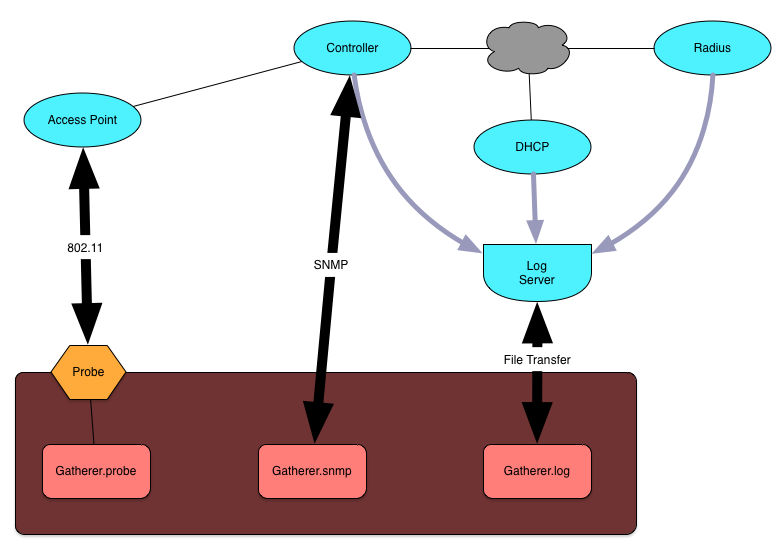
\includegraphics[width=1\linewidth]{Pictures/chapter3/interactions.jpg}
	\caption{Interconnections with the infrastructure}
\end{figure}

\subsection{Controller}
The controller hosts all the \texttt{SNMP} data about itself or the access points. Our system will collect them directly on the controller periodically. As shown, it's the \texttt{gatherer.snmp} that handles the transactions. As said before, there are two controllers hidden behind one virtual IP. That configuration permits to always perform the request to the same address and only the active controller will answer.

\subsection{Access Points}
The probe associates with an access point and the resulting messages are sent to the server. There is no special configuration required as the device needs to operate as a lambda user. The initial configuration of the device, such as the wireless driver, stays unmodified.

\subsection{Log Server} 
The log files are stored on a dedicated server and the administrator retrieves them from there. In an ideal situation, we should automatize the gathering of those files and process them periodically too.
